The default settings for the experiments run in this research are shown in table \ref{tab:default}.

\begin{table}[H]
\begin{tabular}{|l|l|}
\hline
\textbf{Parameter} & \textbf{Default value}\\
\hline
Color space & Opponent\\
SIFT type & Dense\\
Training set size feature histogram & 75 per class\\
Training set size SVM & 75 per class\\
Test set size & 50 per class \\
Cluster size & 400 \\
Step size (only for dense SIFT) & 20\\
\hline
\end{tabular}
\caption{Default values for experiments}
\label{tab:default}
\end{table}

\subsection{Effect of different color spaces in key-point SIFT}

\begin{table}[H]
\begin{tabular}{|c|ccccc|}
\hline
\textbf{Color space} & \textbf{AP Airplanes} & \textbf{AP Cars} & \textbf{AP Faces} & \textbf{AP Motorbikes} & \textbf{MAP}\\
\hline
gray & & & & & \\
normalizedRGB & & & & & \\
RGB & & & & & \\
opponent & & & & & \\
\hline
\end{tabular}
\caption{Effect of different color spaces for key SIFT}
\end{table}


\subsection{Effect of different color spaces in dense SIFT}

\begin{table}[H]
\begin{tabular}{|c|ccccc|}
\hline
\textbf{Color space} & \textbf{AP Airplanes} & \textbf{AP Cars} & \textbf{AP Faces} & \textbf{AP Motorbikes} & \textbf{MAP}\\
\hline
gray & 0.6476 & 0.7741 & 0.4292 & 0.8165 & 0.6668\\
normalizedRGB & 0.5743 & 0.3402 & 0.4678 & 0.5646 & 0.4867\\
RGB & 0.6424 & 0.9726 &  0.8689 & 0.6747 & 0.7897\\
opponent & 0.6447 & 0.9053 & 0.9510 & 0.7516 & 0.8132\\
\hline
\end{tabular}
\caption{Effect of different color spaces for dense SIFT}
\label{tab:color_sift}
\end{table}

Table \ref{tab:color_sift} shows that Opponent SIFT has the highest Mean Average Precision score. The opponent color space is shift-invariant with respect to light intensity and outperforms the classifiers which use gray or RGB color space, which are not invariant. Surprisingly, the classifier which uses the normalized RGB color space performs worst, even though this color space is scale-invariant and invariant to light intensity changes. \\
TODO: WHY??

\cite{van2010evaluating}
\subsection{Effect number of training samples for feature histogram}
\begin{figure}[H]
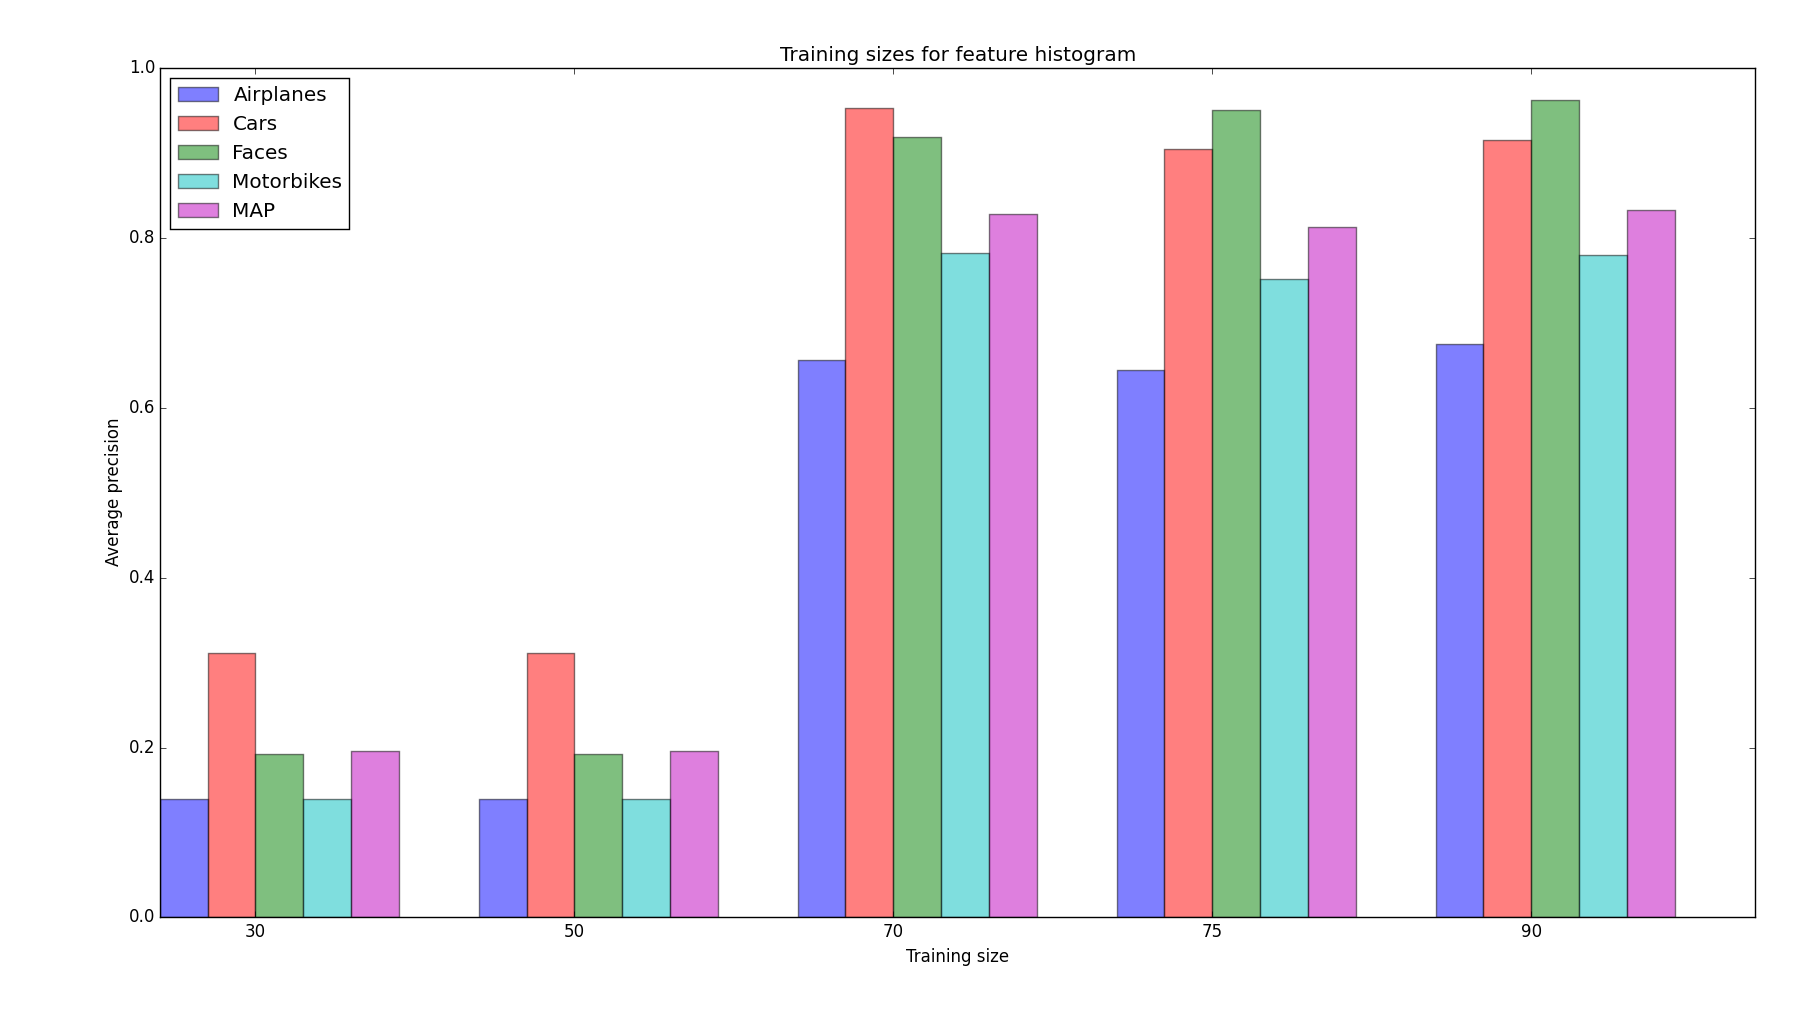
\includegraphics[scale=0.40]{plots/training_size_feature_histograms}
\caption{Effect of training size for histograms on AP}
\end{figure}
\begin{table}[H]
\begin{tabular}{|c|ccccc|}
\hline
\textbf{Training samples} & \textbf{AP Airplanes} & \textbf{AP Cars} & \textbf{AP Faces} & \textbf{AP Motorbikes} & \textbf{MAP}\\
\hline
30 & 0.1394 & 0.3118& 0.1924& 0.1394 & 0.1958\\
50 & 0.1394 & 0.3118& 0.1924& 0.1394 & 0.1958\\
70 & 0.6563 & 0.9534 & 0.9191 & 0.7830 & 0.8280\\
75 & 0.6447 & 0.9053 & 0.9510 & 0.7516 & 0.8132\\
90 & 0.6749 & 0.9157 & 0.9631 & 0.7798 & 0.8334\\
\hline
\end{tabular}
\caption{Effect number of training samples (per class) for feature histogram, Sift type: dense, Color space: opponent}
\end{table}


\subsection{Effect number of training samples for SVM}
\begin{figure}[H]
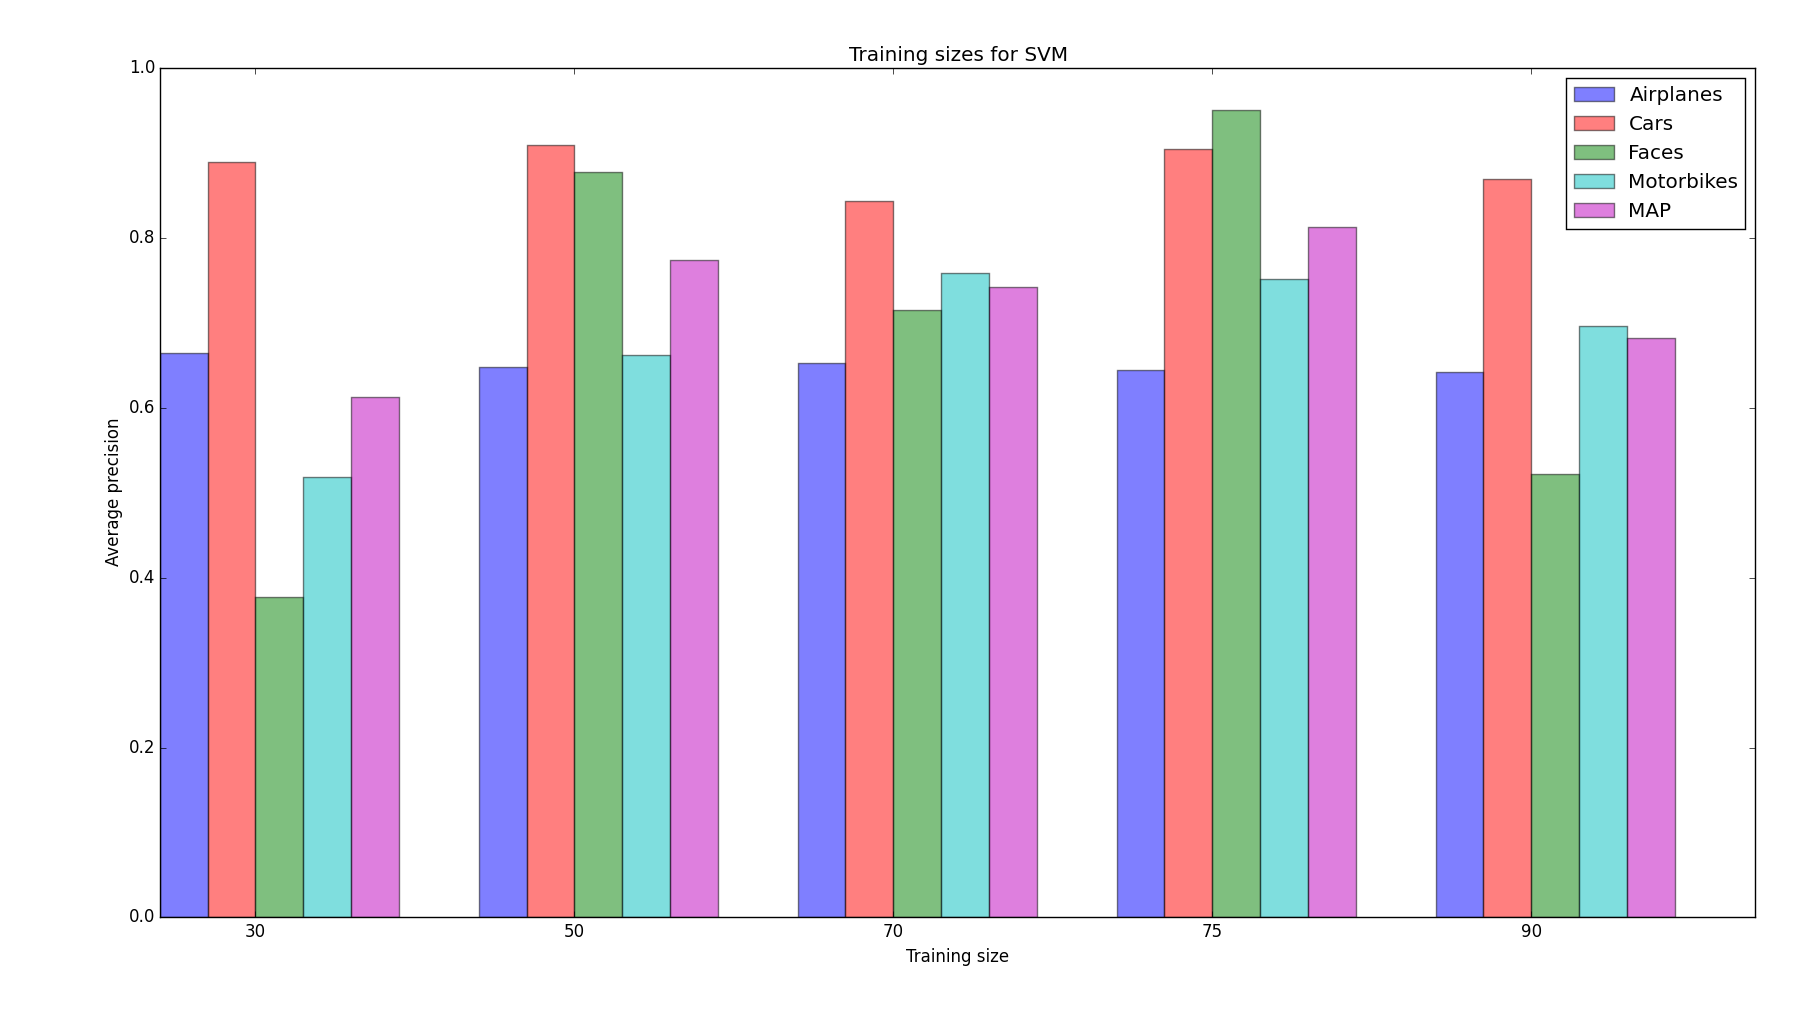
\includegraphics[scale=0.40]{plots/training_size_SVM}
\caption{Effect of training size for SVMs on AP}
\end{figure}

\begin{table}[H]
\begin{tabular}{|c|ccccc|}
\hline
\textbf{Training samples} & \textbf{AP Airplanes} & \textbf{AP Cars} & \textbf{AP Faces} & \textbf{AP Motorbikes} & \textbf{MAP}\\
\hline
30 & 0.6647 & 0.8898 & 0.3772 & 0.5184& 0.6125\\
50 & 0.6484 & 0.9096 & 0.8780 & 0.6627 & 0.7747\\
70 & 0.6531 & 0.8441 & 0.7156 & 0.7590 & 0.7429\\
75 & 0.6447 & 0.9053 & 0.9510 & 0.7516 & 0.8132\\
90 & 0.6426 & 0.8697 & 0.5227 & 0.6963 & 0.6828\\
\hline
\end{tabular}
\caption{Effect number of training samples (per class) for SVM, Sift type: dense, Color space: opponent}
\end{table}


\subsection{Effect of different cluster sizes}

\begin{figure}[H]
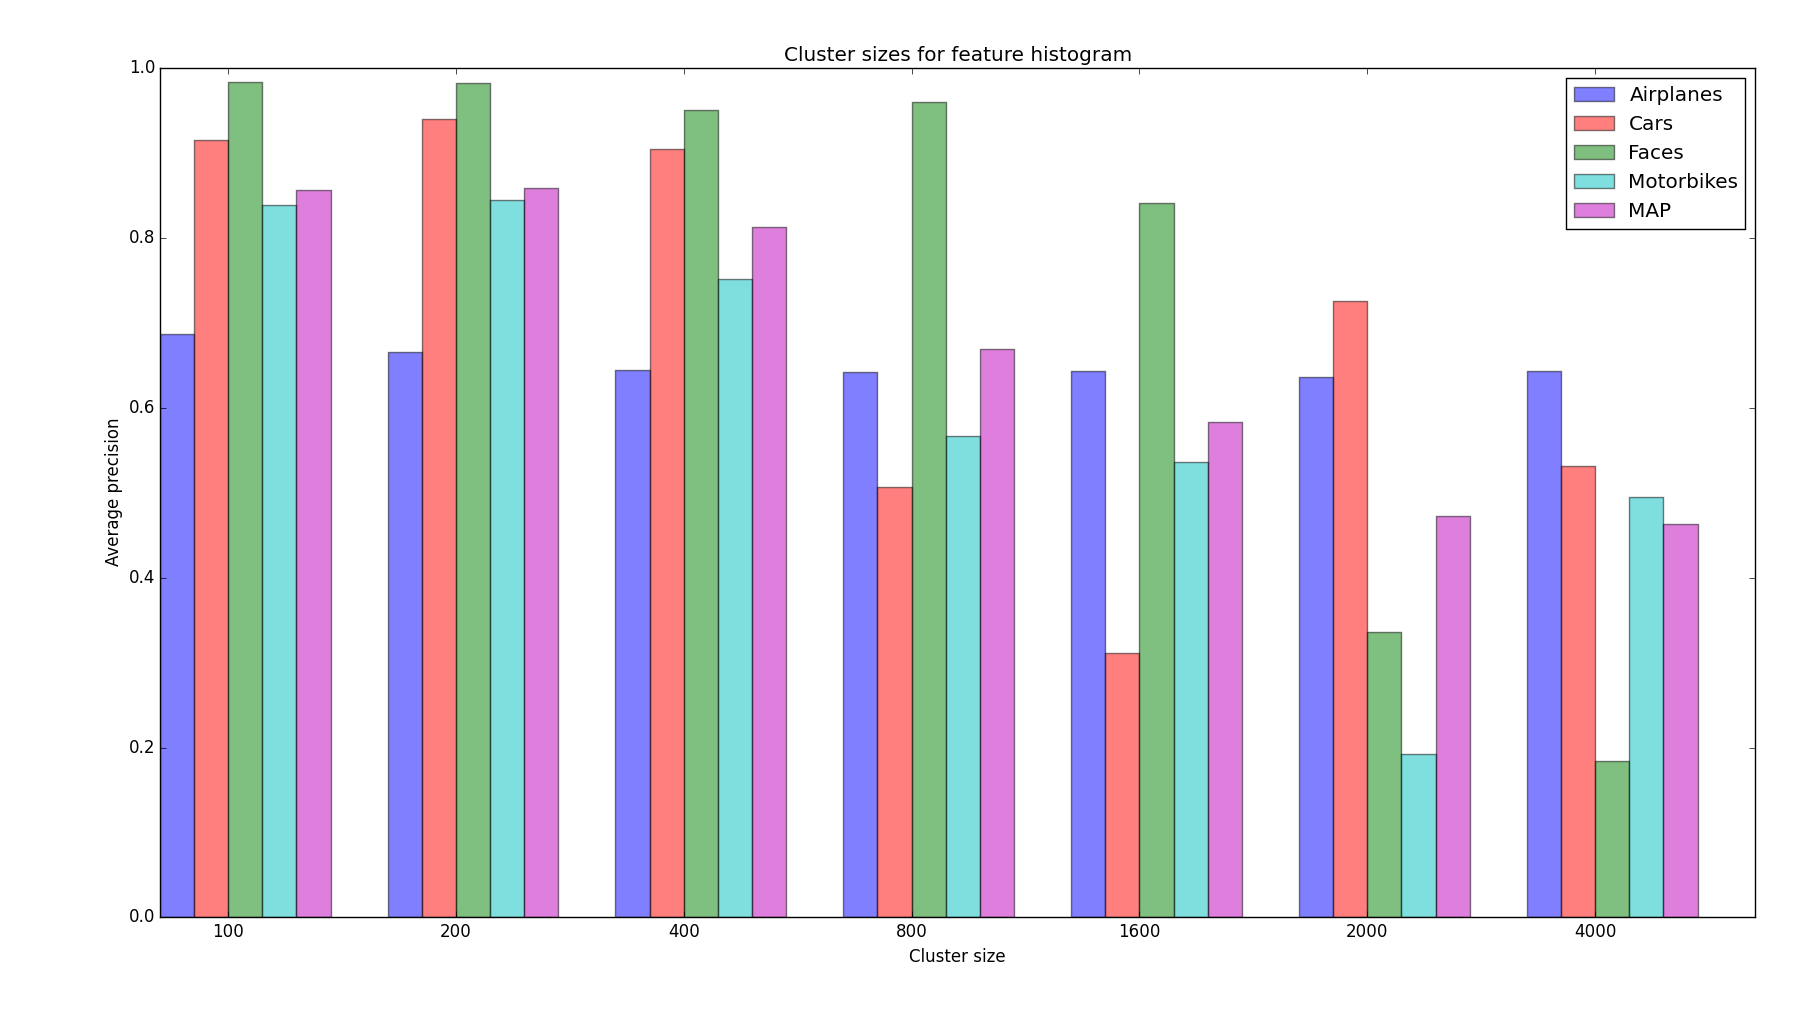
\includegraphics[scale=0.40]{plots/cluster_size_feature_histograms}
\caption{Effect of cluster size on AP}
\end{figure}
\begin{table}[H]
\begin{tabular}{|c|ccccc|}
\hline
\textbf{Cluster size} & \textbf{AP Airplanes} & \textbf{AP Cars} & \textbf{AP Faces} & \textbf{AP Motorbikes} & \textbf{MAP}\\
\hline
100& 0.6868 & 0.9152 & 0.9843 & 0.8395 & 0.8564\\
200 & 0.6663 & 0.9408 & 0.9824 & 0.8454 & 0.8587\\
400 & 0.6447 & 0.9053 & 0.9510 & 0.7516 & 0.8132\\
800 & 0.6424 & 0.5067 & 0.9602 & 0.5667 & 0.6690\\
1600 & 0.6438 & 0.3115 & 0.8410 & 0.5361 & 0.5831\\
2000 & 0.6367 & 0.7253 & 0.3357 & 0.1926 & 0.4726\\
4000 & 0.6430 & 0.5311 & 0.1837 & 0.4956 & 0.4634\\
\hline
\end{tabular}
\caption{Effect of different cluster sizes, Sift type: dense, Color space: opponent}
\end{table}

\subsection{Effect of different step sizes for dense SIFT}
\begin{figure}[H]
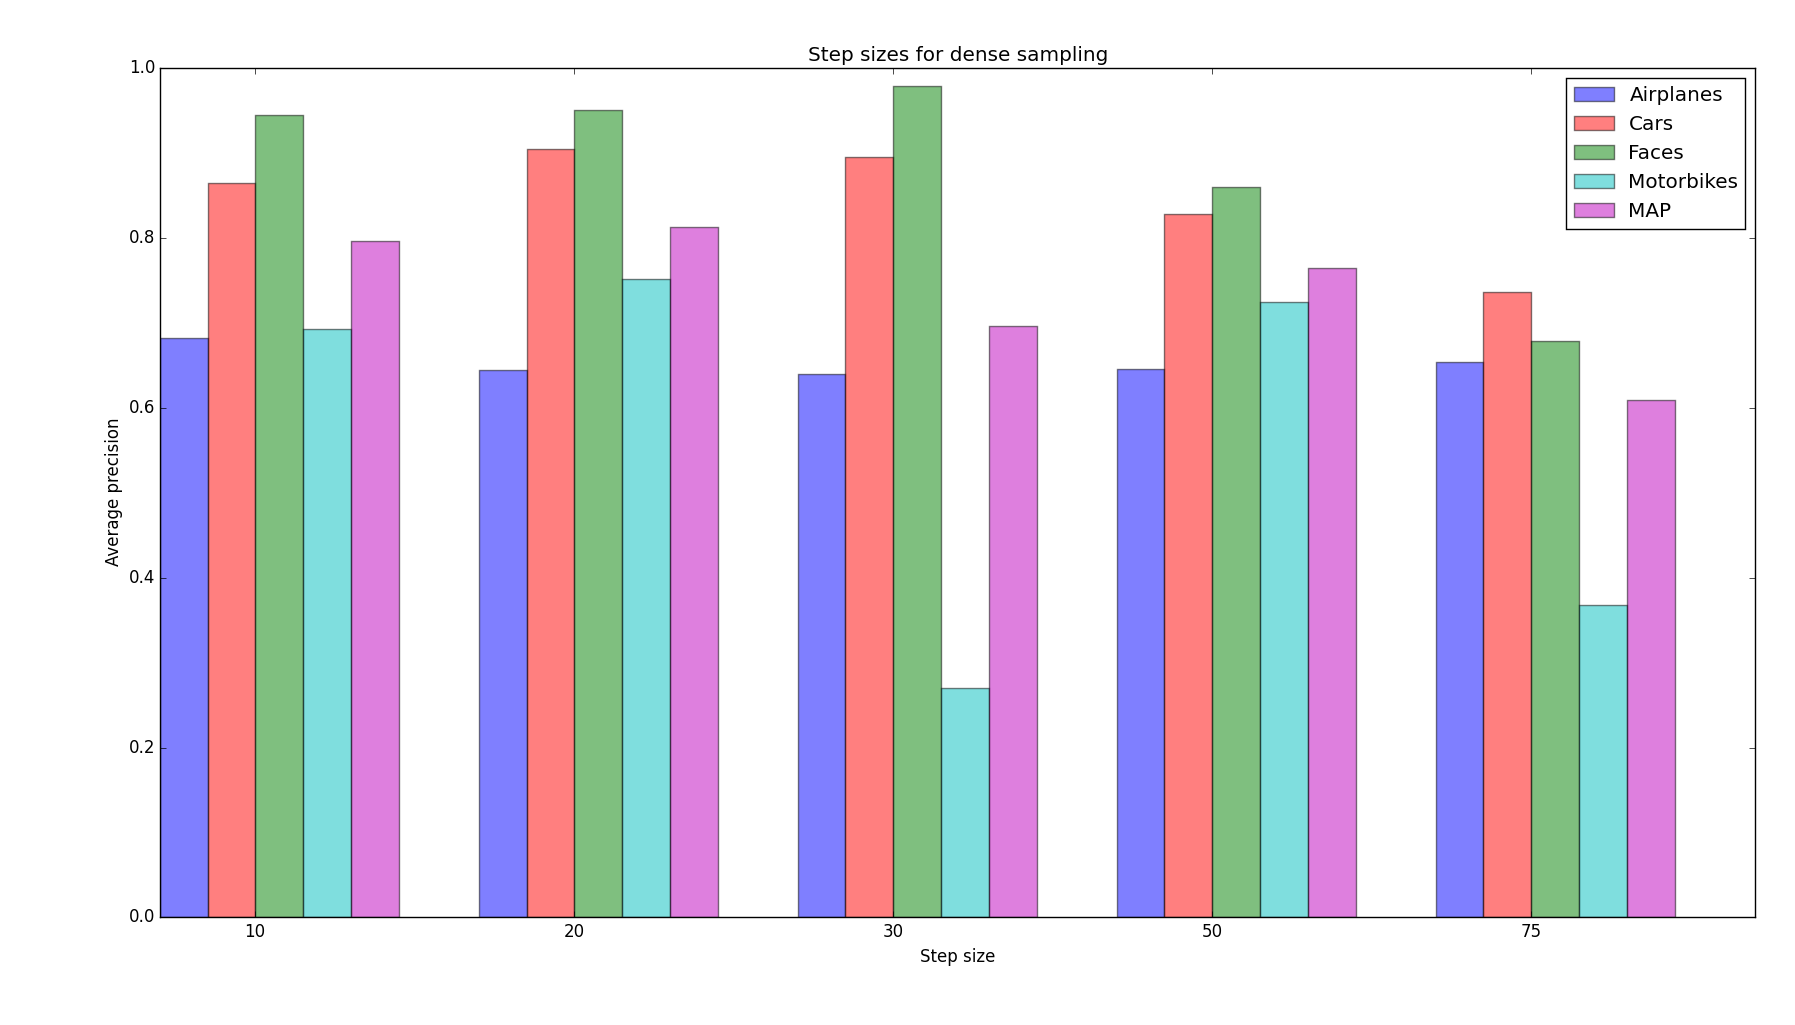
\includegraphics[scale=0.40]{plots/step_sizes_dense_sampling}
\caption{Effect of step size on AP}
\end{figure}
\begin{table}[H]
\begin{tabular}{|c|ccccc|}
\hline
\textbf{Step size} & \textbf{AP Airplanes} & \textbf{AP Cars} & \textbf{AP Faces} & \textbf{AP Motorbikes} & \textbf{MAP}\\
\hline
10 & 0.6823 & 0.8654 & 0.9444 & 0.6934 & 0.7964\\
20 & 0.6447 & 0.9053 & 0.9510 & 0.7516 & 0.8132\\
30 & 0.6405 &  0.8952& 0.9792& 0.2704 & 0.6963\\
50 & 0.6463 & 0.8288 & 0.8596 & 0.7247 & 0.7648\\
75 & 0.6539 & 0.7360 & 0.6791 & 0.3673 & 0.6091\\
\hline
\end{tabular}
\caption{Effect of different step sizes for dense SIFT Color space: opponent}
\end{table}



\subsection{Effect of different window sizes for dense SIFT}

\begin{table}[H]
\begin{tabular}{|c|ccccc|}
\hline
\textbf{Window size} & \textbf{AP Airplanes} & \textbf{AP Cars} & \textbf{AP Faces} & \textbf{AP Motorbikes} & \textbf{MAP}\\
\hline
4, 8 & 0.6447 & 0.9053 & 0.9510 & 0.7516 & 0.8132\\
4, 12 & 0.6809 & 0.9505 & 0.9945 & 0.8955 & 0.8803\\
8, 12 & 0.7066 & 0.9031 & 0.9839 & 0.7216 & 0.8288\\
12, 16 & & & & & \\
4, 8, 12 & & & & & \\
8, 12, 16 & & & & & \\
\hline
\end{tabular}
\caption{Effect of different window sizes for dense SIFT,  Color space: opponent}
\end{table}




\subsection{Effect different kernels for SVM}

\begin{table}[H]
\begin{tabular}{|c|ccccc|}
\hline
\textbf{Kernel} & \textbf{AP Airplanes} & \textbf{AP Cars} & \textbf{AP Faces} & \textbf{AP Motorbikes} & \textbf{MAP}\\
\hline
sigmoid & 0.6447 & 0.9053 & 0.9510 & 0.7516 & 0.8132\\
linear & 0.6574 & 0.9668 & 0.9860 & 0.8642 & 0.8686 \\
polynomial & 0.7066 & 0.9031 & 0.9839& 0.7216& 0.8288\\
radial & & & & & \\
\hline
\end{tabular}
\caption{Effect different kernels for SVM, Sift type: dense, Color space: opponent}
\end{table}
